\documentclass{standalone}

\usepackage{tikz}

\begin{document}

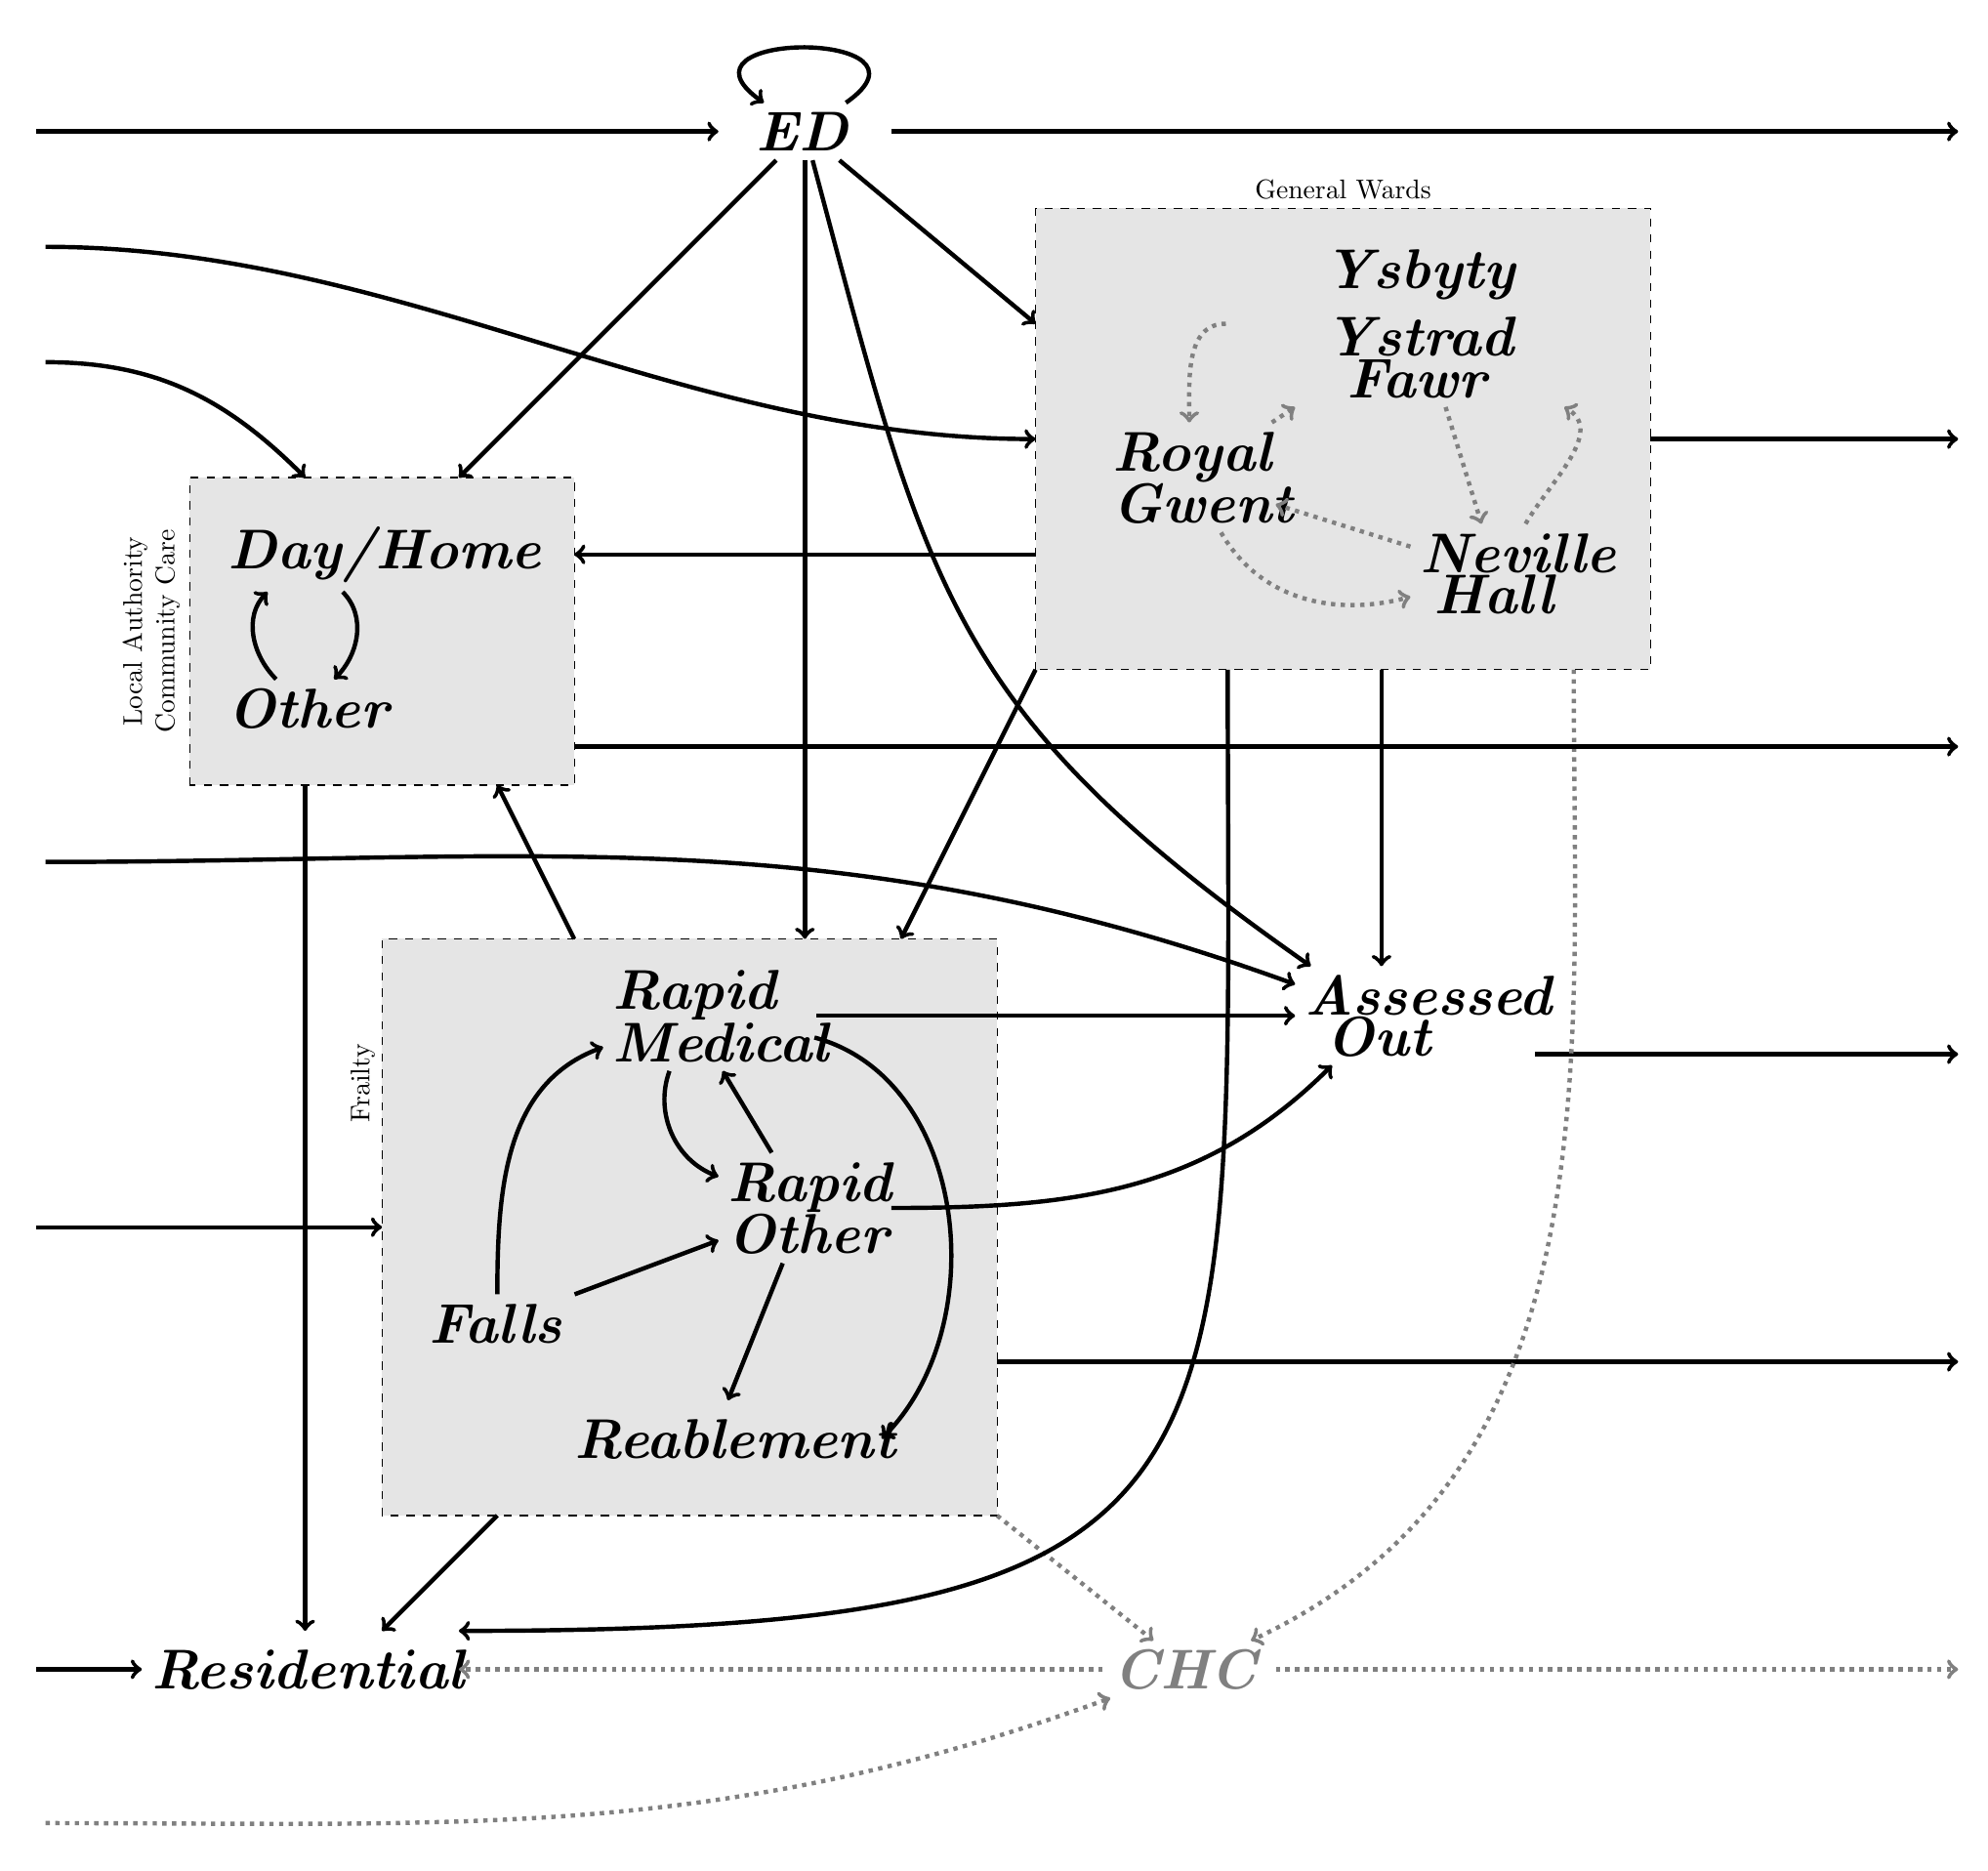
\begin{tikzpicture}

\draw[draw=black, fill=gray!20, dashed] (4.5, -1) rectangle (12.5, 6.5);
\draw[draw=black, fill=gray!20, dashed] (2, 8.5) rectangle (7, 12.5);
\draw[draw=black, fill=gray!20, dashed] (13, 10) rectangle (21, 16);

\node[text width=2cm, align=center] (AE) at (10, 17) {\huge{\textbf{\textit{ED}}}};
\node[text width=2cm, align=center] (RPDM) at (8.5, 5.5) {\huge{\textbf{\textit{Rapid\\Medical}}}};
\node[text width=2cm, align=center] (RPDO) at (10, 3) {\huge{\textbf{\textit{Rapid\\Other}}}};
\node[text width=2cm, align=center] (RG) at (15, 12.5) {\huge{\textbf{\textit{Royal\\Gwent}}}};
\node[text width=2cm, align=center] (NH) at (19, 11.25) {\huge{\textbf{\textit{Neville\\Hall}}}};
\node[text width=4.8cm, align=center] (YYF) at (18, 14.5) {\huge{\textbf{\textit{Ysbyty Ystrad\\Fawr}}}};
\node[text width=2cm, align=center] (AO) at (17.5, 5.5) {\huge{\textbf{\textit{Assessed\\Out}}}};
\node[text width=2cm, align=center] (FLS) at (6, 1.5) {\huge{\textbf{\textit{Falls}}}};
\node[text width=2cm, align=center] (RBL) at (8, 0) {\huge{\textbf{\textit{Reablement}}}};
\node[text width=2cm, align=center, text=gray] (CHC) at (15, -3) {\huge{\textbf{\textit{CHC}}}};
\node[text width=2cm, align=center] (CCD) at (3.5, 11.5) {\huge{\textbf{\textit{Day/Home}}}};
\node[text width=2cm, align=center] (CCO) at (3.5, 9.5) {\huge{\textbf{\textit{Other}}}};
\node[text width=2cm, align=center] (RES) at (2.5, -3) {\huge{\textbf{\textit{Residential}}}};
\node (LAIN) at (0, 14) {};
\node (CHCIN) at (0, -5) {};
\node (EMOUTC) at (20, 10.125) {};
\node (EMOUTR) at (15.5, 10.125) {};
\node (EMOUTA) at (17.5, 10.125) {};
\node (EMIN) at (0, 15.5) {};
\node (AOIN) at (0, 7.5) {};
\node (RPDMOUT) at (10, 5.25) {};

\draw[ultra thick, ->] (AE) -- (13, 14.5);
\draw[ultra thick, ->] (AE) edge[out=-75, in=145, looseness=1.2] (AO);
\draw[ultra thick, ->] (10.15, 5.5) -- (AO);
\draw[ultra thick, ->] (AE) -- (10, 6.5);
\draw[ultra thick, ->] (0, 2.75) -- (4.5, 2.75);
\draw[ultra thick, ->] (21, 13) -- (25, 13);
\draw[ultra thick, ->] (19.5, 5) -- (25, 5);
\draw[gray, ultra thick, ->, dotted] (CHCIN) edge[out=0, in=-160] (CHC);
\draw[gray, ultra thick, ->, dotted] (CHC) -- (25, -3);
\draw[ultra thick, ->] (13, 10) -- (11.25, 6.5);
\draw[ultra thick, ->] (RPDMOUT) edge[out=-15, in=45] (11, 0);
\draw[ultra thick, ->] (RPDO) -- (9, 0.5);
\draw[ultra thick, ->] (RPDO) -- (RPDM);
\draw[ultra thick, ->] (RPDM) edge[out=-110, in=160] (RPDO);
\draw[ultra thick, ->] (12.5, 1) -- (25, 1);
\draw[gray, ultra thick, ->, dotted] (12.5, -1) -- (CHC);
\draw[gray, ultra thick, ->, dotted] (EMOUTC) edge[out=-90, in=25] (CHC);
\draw[ultra thick, ->] (FLS) edge[out=90, in=-160] (RPDM);
\draw[ultra thick, ->] (FLS) -- (RPDO);
\draw[ultra thick, ->] (0, 17) -- (AE);
\draw[ultra thick, ->] (AE) -- (25, 17);
\draw[ultra thick, ->] (AE) edge[out=35, in=145, looseness=4] (AE);
\draw[ultra thick, ->] (CCD) edge[out=-45, in=45] (CCO);
\draw[ultra thick, ->] (CCO) edge[out=135, in=-135] (CCD);
\draw[ultra thick, ->] (AE) -- (5.5, 12.5);
\draw[ultra thick, ->] (13, 11.5) -- (7, 11.5);
\draw[gray, ultra thick, ->, dotted] (CHC) -- (5.5, -3);
\draw[ultra thick, ->] (3.5, 8.5) -- (3.5, -2.5);
\draw[ultra thick, ->] (6, -1) -- (4.5, -2.5);
\draw[ultra thick, ->] (EMOUTR) edge[out=-90, in=0, looseness=1.7] (5.5, -2.5);
\draw[ultra thick, ->] (7, 6.5) -- (6, 8.5);
\draw[ultra thick, ->] (LAIN) edge[out=0, in=135] (3.5, 12.5);
\draw[ultra thick, ->] (7, 9) -- (25, 9);
\draw[ultra thick, ->] (0, -3) -- (RES);
\draw[ultra thick, ->] (EMIN) edge[out=0, in=180, looseness=0.9] (13, 13);
\draw[ultra thick, ->] (AOIN) edge[out=0, in=160] (AO);
\draw[ultra thick, ->] (RPDO) edge[out=0, in=-135] (AO);
\draw[ultra thick, ->] (EMOUTA) -- (AO);
\draw[gray, ultra thick, ->, dotted] (RG) -- (YYF);
\draw[gray, ultra thick, ->, dotted] (YYF) -- (NH);
\draw[gray, ultra thick, ->, dotted] (NH) -- (RG);
\draw[gray, ultra thick, ->, dotted] (RG) edge[out=-60, in=-165] (NH);
\draw[gray, ultra thick, ->, dotted] (YYF) edge[out=180, in=90] (RG);
\draw[gray, ultra thick, ->, dotted] (NH) edge[out=60, in=-30] (YYF);


\node[rotate=90, align=center] at (1.5, 10.5) {\normalsize{Local Authority}\\\normalsize{Community Care}};
\node[rotate=90, align=center] at (4.25, 4.625) {\normalsize{Frailty}};
\node[align=center] at (17, 16.25) {\normalsize{General Wards}};

\end{tikzpicture}

\end{document}
